
\begin{figure}[t]
  \centering
  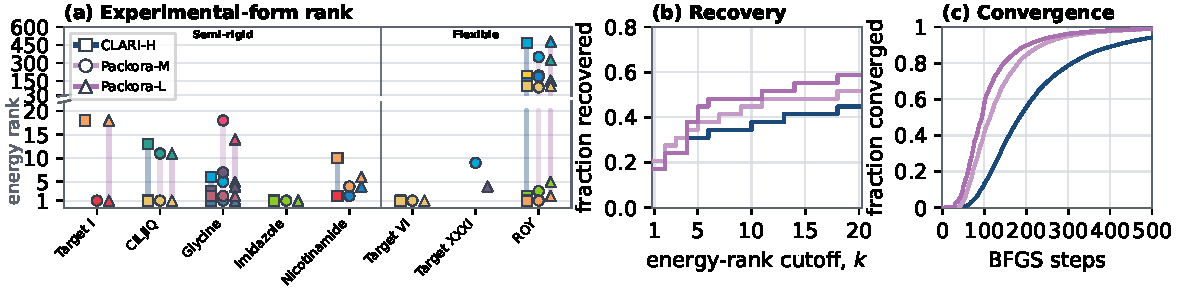
\includegraphics[width=\textwidth]{figures/generated/fig_fastcsp_multi_ranking.pdf}
  \caption{\textbf{FastCSP multi-polymorph benchmark.}
    We generate 1{,}000 candidates for each of the 29 target structures
    across eight systems, relax them with
    UMA-S-1.2~\citep{wood2025family}, and rank them by increasing energy within
    each system. \textbf{(a)} Best energy rank of each of the 29 polymorphs
    for CLARI-H, \model{}-M, and \model{}-L; lower is better, with rank
    1 denoting the predicted minimum-energy structure. Marker color identifies
    the polymorph across systems. \model{}-L and \model{}-M recover
    21 and 19 polymorphs, respectively,
    compared with 18 for CLARI-H. \textbf{(b)} Fraction of
    polymorphs recovered by energy-rank cutoff $k$; \model{} achieves higher
    recovery across cutoffs. \textbf{(c)} Cumulative fraction of the generated candidates converged by BFGS step; \model{} candidates converge faster throughout relaxation.
    Relaxing all candidates on eight NVIDIA H200 GPUs takes 16.8, 10.6, and
    8.9~h for CLARI-H, \model{}-M, and \model{}-L, respectively.}
  \label{fig:fastcsp-multi-ranking}
\end{figure}
